% =====================================================================
%  Лабораторная работа №2. Методы решения нелинейных уравнений.
%  Вариант 4: x^3 - 0.1 x^2 + 0.4 x - 1.5 = 0.
%
%  Сборка (любой из вариантов):
%      pdflatex  BastrakovReport.tex
%      xelatex   BastrakovReport.tex
%      lualatex  BastrakovReport.tex
%  (запускать два раза — для оглавления и перекрёстных ссылок)
% =====================================================================
\documentclass[14pt,a4paper]{extarticle}

% - Поддержка кириллицы: pdfLaTeX (T2A) либо XeLaTeX/LuaLaTeX (fontspec) -
\usepackage{iftex}
\ifPDFTeX
    \usepackage[T2A]{fontenc}
    \usepackage[utf8]{inputenc}
    \usepackage[russian]{babel}
    \usepackage{tempora}                 % гарнитура Times с кириллицей
    \usepackage{listingsutf8}            % кириллица внутри листингов
\else
    \usepackage{fontspec}
    \usepackage{polyglossia}
    \setdefaultlanguage{russian}
    \setotherlanguage{english}
    % Каскад шрифтов: сначала системные (есть кириллица), потом TeX Gyre
    \IfFontExistsTF{Liberation Serif}%
        {\setmainfont{Liberation Serif}}%
        {\IfFontExistsTF{PT Serif}%
            {\setmainfont{PT Serif}}%
            {\setmainfont{TeX Gyre Termes}}}
    \IfFontExistsTF{DejaVu Sans Mono}%
        {\setmonofont{DejaVu Sans Mono}}%
        {\IfFontExistsTF{Liberation Mono}%
            {\setmonofont{Liberation Mono}}%
            {\setmonofont{TeX Gyre Cursor}}}
\fi

% - Математика, графика, оформление -----------
\usepackage{amsmath,amssymb}
\usepackage{graphicx}
\usepackage{geometry}
\usepackage{booktabs}
\usepackage{array}
\usepackage{float}
\usepackage{caption}
\usepackage{indentfirst}
\usepackage{xcolor}
\usepackage{listings}
\usepackage[hidelinks]{hyperref}

\geometry{a4paper,left=3cm,right=1.5cm,top=2cm,bottom=2cm}
\graphicspath{{graphics/img/}}

\captionsetup{labelsep=endash,justification=centering}
\setlength{\parindent}{1.25cm}
\renewcommand{\arraystretch}{1.15}
\renewcommand{\labelenumi}{\arabic{enumi})}

% - Настройка листингов ---------------
\definecolor{lstgray}{gray}{0.45}
\definecolor{lstgreen}{rgb}{0.0,0.45,0.0}
\definecolor{lstblue}{rgb}{0.05,0.15,0.55}
\definecolor{lstred}{rgb}{0.6,0.1,0.1}

\lstset{
    basicstyle=\ttfamily\footnotesize,
    language={[Sharp]C},
    breaklines=true,
    frame=single,
    numbers=left,
    numberstyle=\tiny\color{lstgray},
    keywordstyle=\color{lstblue}\bfseries,
    commentstyle=\color{lstgreen}\itshape,
    stringstyle=\color{lstred},
    showstringspaces=false,
    tabsize=4,
    captionpos=b,
    columns=fullflexible,
    keepspaces=true,
}

% Подключение файла с исходным кодом (у pdfLaTeX кириллица через listingsutf8;
% признак \lst@UseInputEncoding вводится пакетом listingsutf8)
\newcommand{\includecode}[1]{%
    \ifPDFTeX
        \ifcsname lst@UseInputEncoding\endcsname
            \lstinputlisting[inputencoding=utf8]{#1}%
        \else
            \lstinputlisting{#1}%
        \fi
    \else
        \lstinputlisting{#1}%
    \fi
}

\begin{document}

% =====================================================================
%  Титульный лист
% =====================================================================
\begin{titlepage}
    \centering
    \large
    Министерство образования и науки РФ\\[0.3cm]
    Пермский национальный исследовательский политехнический университет\\[0.3cm]
    Электротехнический факультет\\[0.3cm]
    Кафедра "Информационные технологии и автоматизированные системы"

    \vspace{3.5cm}
    {\Large Информатика в приложении к отрасли}\\[0.4cm]
    {\Large\bfseries Лабораторная работа № 2}\\[0.6cm]

    Тема: "Методы решения нелинейных уравнений"\\[0.2cm]
    Вариант 4

    \vspace{4.5cm}
    \begin{flushleft}
        \large
        Выполнил: студент группы РИС-25-2б \hfill Бастраков Данил\\[0.5cm]
        Проверил: профессор кафедры ИТАС \hfill Шварц К.~Г.\\[0.5cm]
        Дата: \underline{\hspace{7cm}}
    \end{flushleft}

    \vfill
    Пермь\\ 2026
\end{titlepage}

\tableofcontents
\newpage

% =====================================================================
\section{Постановка задачи}
% =====================================================================

\textbf{Цель работы} - отделить корни нелинейного уравнения и уточнить их
с заданной точностью методами половинного деления, хорд, касательных
(Ньютона), комбинированным методом хорд и касательных, а также методом
простых итераций.

Дано нелинейное уравнение (вариант~4):
\begin{equation}
    f(x) = x^3 - 0{,}1\,x^2 + 0{,}4\,x - 1{,}5 = 0.
    \label{eq:main}
\end{equation}

Требуется:
\begin{enumerate}
    \item отделить корни уравнения аналитически;
    \item уточнить корень каждым из указанных методов с точностью
          $\varepsilon = 10^{-6}$;
    \item обосновать выбор начального приближения и проверить условия
          сходимости методов;
    \item привести программную реализацию, сводную таблицу результатов
          и сравнить методы по числу шагов и характеру приближения.
\end{enumerate}

% =====================================================================
\section{Отделение корней}
% =====================================================================

Обозначим $f(x) = x^3 - 0{,}1x^2 + 0{,}4x - 1{,}5$. Найдём первую
производную:
\begin{equation}
    f'(x) = 3x^2 - 0{,}2x + 0{,}4 .
\end{equation}
Дискриминант этого квадратного трёхчлена равен
\begin{equation}
    D = (-0{,}2)^2 - 4\cdot 3 \cdot 0{,}4 = 0{,}04 - 4{,}8 = -4{,}76 < 0,
\end{equation}
поэтому $f'(x) > 0$ при всех $x$. Функция строго возрастает и уравнение
\eqref{eq:main} имеет \emph{ровно один} действительный корень.

Составим таблицу знаков функции (табл.~\ref{tab:signs}).

\begin{table}[H]
    \centering
    \caption{Знаки функции $f(x)$ на грубой сетке}
    \label{tab:signs}
    \begin{tabular}{c|ccccc}
        \toprule
        $x$    & $-2$ & $-1$ & $0$ & $1$ & $2$\\
        \midrule
        $f(x)$ & $-10{,}7$ & $-3{,}0$ & $-1{,}5$ & $-0{,}2$ & $6{,}9$\\
        знак   & $-$ & $-$ & $-$ & $-$ & $+$\\
        \bottomrule
    \end{tabular}
\end{table}

Смена знака происходит на отрезке $[1;2]$, значит $\xi \in [1;2]$.
Уменьшим отрезок, исследуя его с шагом~$0{,}1$:
\[
    f(1{,}0) = -0{,}2 < 0, \qquad f(1{,}1) = 0{,}15 > 0,
\]
откуда \boxed{\xi \in [1;\; 1{,}1]}. Дальнейшее уточнение этого отрезка
и выполняют численные методы.

Вторая производная
\begin{equation}
    f''(x) = 6x - 0{,}2
\end{equation}
на отрезке $[1;1{,}1]$ положительна ($f''(x) > 0$), то есть функция
выпукла вниз. Знак второй производной используется ниже при выборе
начального приближения для методов хорд и касательных.

График функции приведён на рис.~\ref{fig:function}, а расположение корня
на отрезке $[1;1{,}1]$ - на рис.~\ref{fig:separation}.

\begin{figure}[H]
    \centering
    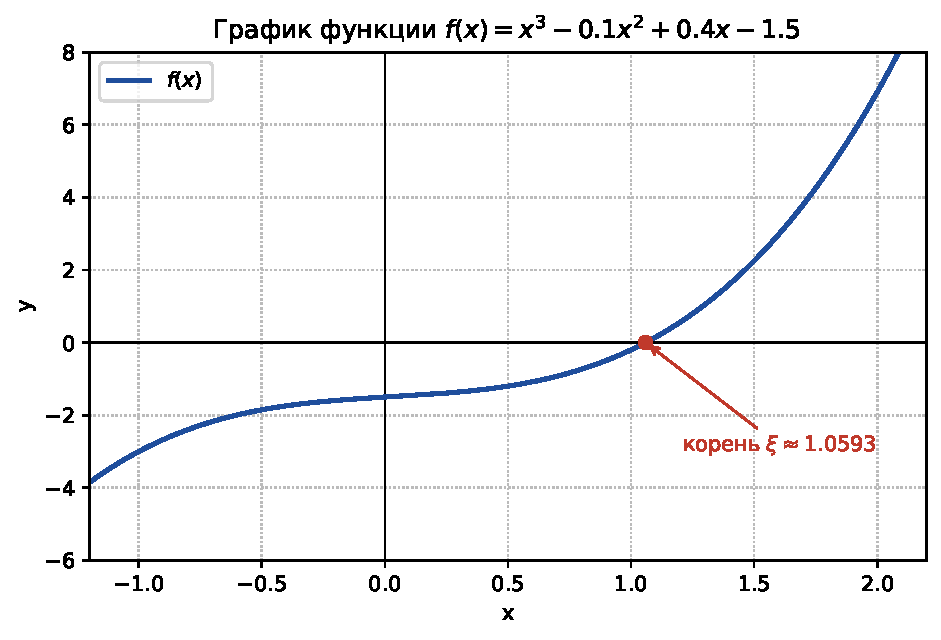
\includegraphics[width=0.86\textwidth]{fig_function.pdf}
    \caption{График функции $f(x)=x^3-0{,}1x^2+0{,}4x-1{,}5$}
    \label{fig:function}
\end{figure}

\begin{figure}[H]
    \centering
    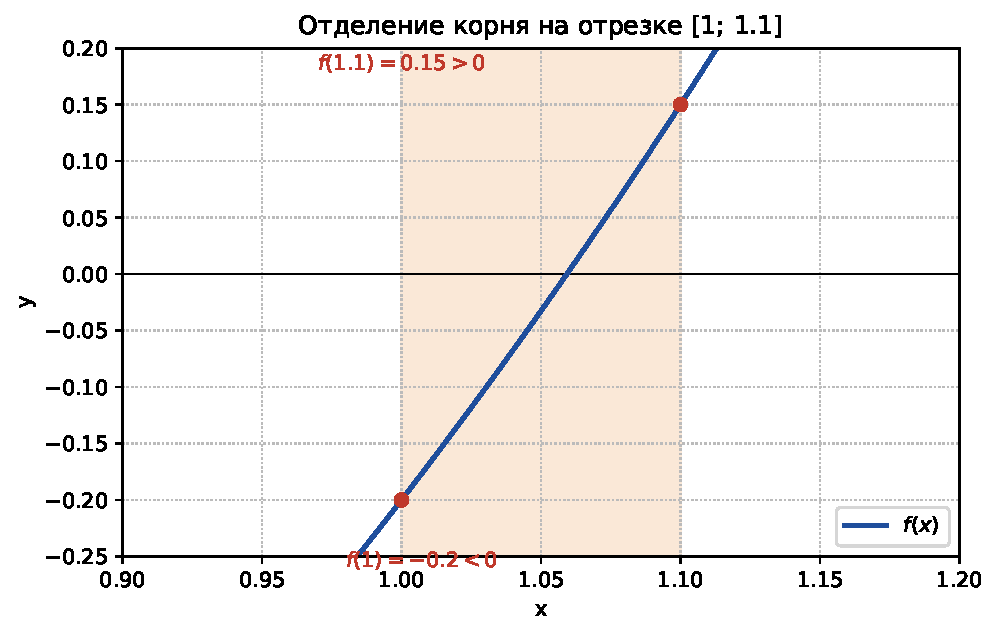
\includegraphics[width=0.86\textwidth]{fig_separation.pdf}
    \caption{Отделение корня на отрезке $[1;1{,}1]$}
    \label{fig:separation}
\end{figure}

% =====================================================================
\section{Краткое описание методов}
% =====================================================================

Все методы уточнения корня применяются к отрезку $[a;b]$, на концах
которого функция принимает значения разных знаков: $f(a)\cdot f(b) < 0$.

\subsection{Метод половинного деления (дихотомии)}

Отрезок $[a;b]$ делится пополам точкой $c=(a+b)/2$. Из двух половин
выбирается та, на концах которой знаки функции различны:
\begin{equation}
    \text{если } f(a)\cdot f(c)\le 0, \text{ то } b:=c, \quad
    \text{иначе } a:=c .
\end{equation}
После $n$ делений длина отрезка равна $(b-a)/2^{\,n}$, поэтому метод
сходится всегда и со скоростью геометрической прогрессии со
знаменателем $1/2$. Условие останова: $b-a < \varepsilon$. Приближение
к корню идёт с двух сторон: левые концы $a_n$ не убывают, правые $b_n$
не возрастают (рис.~\ref{fig:bisection}).

\begin{figure}[H]
    \centering
    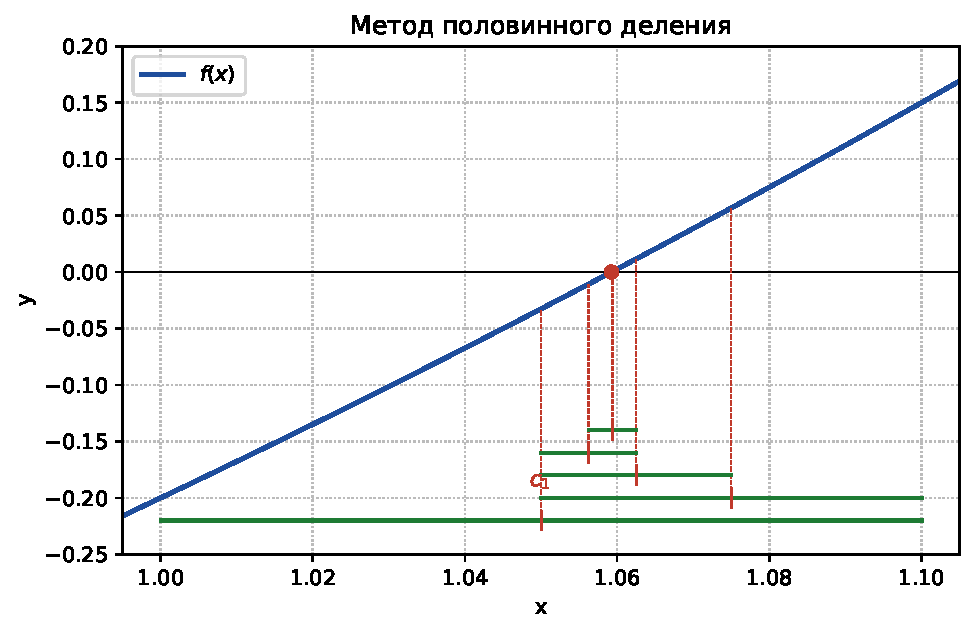
\includegraphics[width=0.8\textwidth]{fig_bisection.pdf}
    \caption{Метод половинного деления: последовательное деление отрезка}
    \label{fig:bisection}
\end{figure}

\subsection{Метод хорд}

Проводится хорда через точки $(a,f(a))$ и $(b,f(b))$; точка её
пересечения с осью $Ox$ принимается за новое приближение. Один конец
отрезка неподвижен - это тот, для которого $f(x)\cdot f''(x) > 0$;
начальным приближением служит противоположный конец. В нашем случае
$f(b)\cdot f''(b) > 0$, поэтому неподвижен конец $b$, а $x_0 = a$:
\begin{equation}
    x_{n+1} = x_n - \frac{f(x_n)}{f(b) - f(x_n)}\,(b - x_n).
    \label{eq:chord}
\end{equation}
Последовательность монотонна и приближается к корню с одной стороны
(рис.~\ref{fig:chord}). Скорость сходимости - линейная.

\begin{figure}[H]
    \centering
    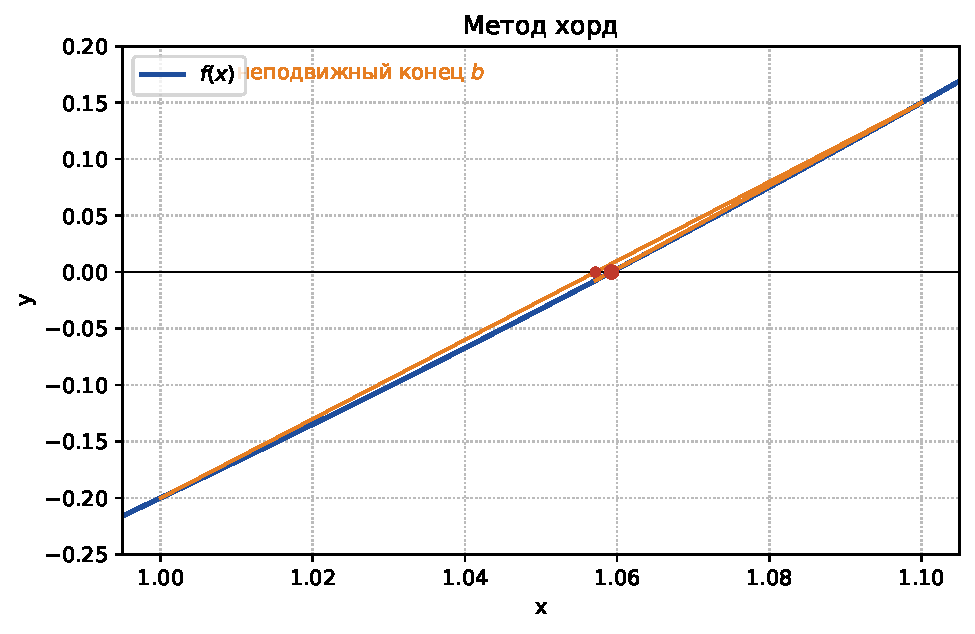
\includegraphics[width=0.8\textwidth]{fig_chord.pdf}
    \caption{Метод хорд: приближение с одной стороны}
    \label{fig:chord}
\end{figure}

\subsection{Метод касательных (Ньютона)}

В точке $x_n$ проводится касательная к графику функции; точка её
пересечения с осью $Ox$ даёт следующее приближение:
\begin{equation}
    x_{n+1} = x_n - \frac{f(x_n)}{f'(x_n)} .
    \label{eq:newton}
\end{equation}
За начальное приближение выбирается тот конец отрезка, где
$f(x_0)\cdot f''(x_0) > 0$ (условие сходимости Фурье). В нашем случае
$x_0 = b = 1{,}1$. Метод имеет квадратичную сходимость и приближается к
корню с одной стороны (рис.~\ref{fig:newton}).

\begin{figure}[H]
    \centering
    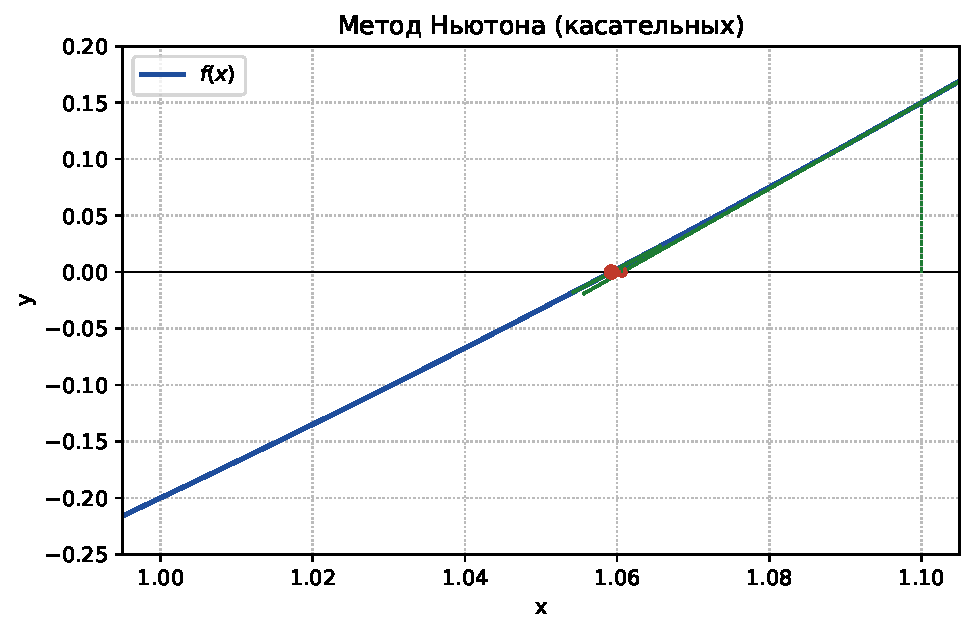
\includegraphics[width=0.8\textwidth]{fig_newton.pdf}
    \caption{Метод касательных: построение касательных}
    \label{fig:newton}
\end{figure}

\subsection{Комбинированный метод хорд и касательных}

Корень уточняется одновременно с двух сторон. Обозначим $x_n$ -
приближение по недостатку (методом хорд), $y_n$ - по избытку (методом
касательных). Хорды строятся из конца, где $f(x)\cdot f''(x) < 0$, а
касательные - из конца, где $f(x)\cdot f''(x) > 0$. Тогда
\begin{equation}
    x_{n+1} = x_n - \frac{f(x_n)}{f(x_n)-f(y_n)}\,(x_n - y_n), \qquad
    y_{n+1} = y_n - \frac{f(y_n)}{f'(y_n)} .
    \label{eq:combined}
\end{equation}
Процесс заканчивается при $y_n - x_n < \varepsilon$; корень всегда
заключён между $x_n$ и $y_n$ (рис.~\ref{fig:combined}). Метод даёт
оценку погрешности на каждом шаге и сходится быстрее метода хорд.

\begin{figure}[H]
    \centering
    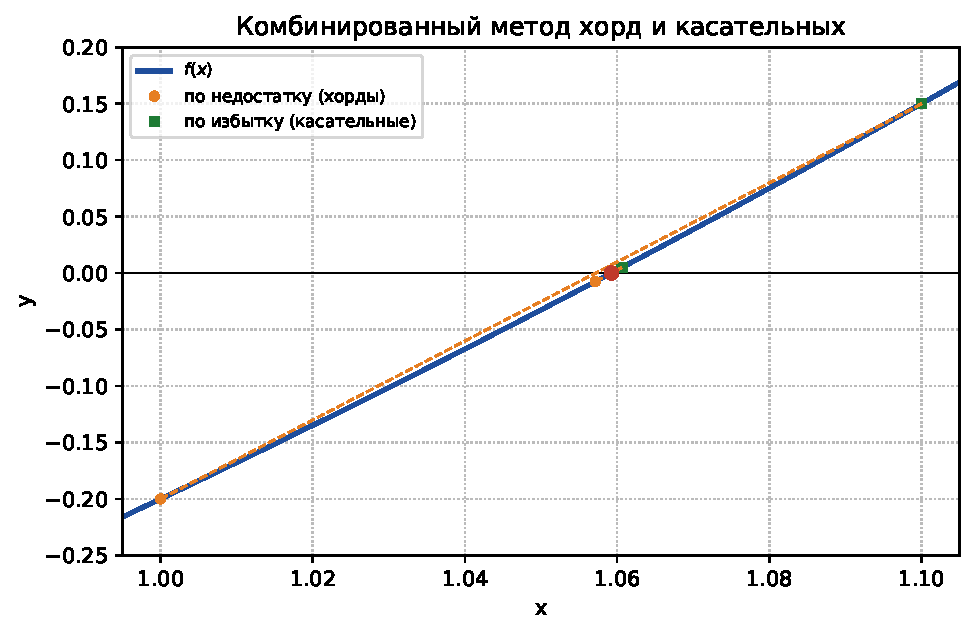
\includegraphics[width=0.82\textwidth]{fig_combined.pdf}
    \caption{Комбинированный метод: хорды слева, касательные справа}
    \label{fig:combined}
\end{figure}

\subsection{Метод простых итераций}

Уравнение $f(x)=0$ приводится к виду $x=\varphi(x)$. Возьмём
\begin{equation}
    \varphi(x) = x - \frac{f(x)}{k},
\end{equation}
где параметр $k$ выбирается одного знака с $f'(x)$ и по модулю больше
$Q/2$, а $Q=\max_{[a;b]}|f'(x)|$. Тогда
\begin{equation}
    \varphi'(x) = 1 - \frac{f'(x)}{k}, \qquad
    |\varphi'(x)| \le q < 1,
\end{equation}
что обеспечивает сходимость последовательности $x_{n+1}=\varphi(x_n)$.
Оценка погрешности:
\begin{equation}
    |\xi - x_n| \le \frac{q}{1-q}\,|x_n - x_{n-1}| .
\end{equation}
Приближения подходят к корню с одной стороны (лестница) при
$\varphi'(x)>0$ (рис.~\ref{fig:iteration}).

\begin{figure}[H]
    \centering
    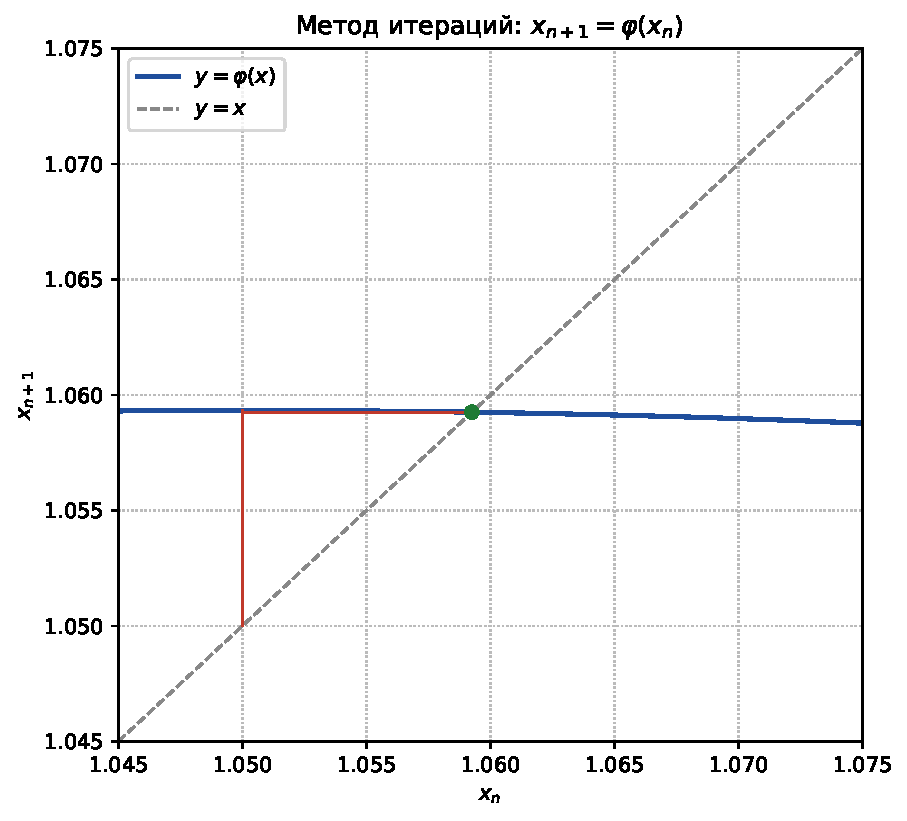
\includegraphics[width=0.66\textwidth]{fig_iteration.pdf}
    \caption{Метод итераций: лестница приближений к корню}
    \label{fig:iteration}
\end{figure}

% =====================================================================
\section{Проверка условий сходимости и выбор начального приближения}
% =====================================================================

На отрезке $[1;1{,}1]$ имеем $f(1) = -0{,}2 < 0$, $f(1{,}1)=0{,}15>0$,
$f''(x)=6x-0{,}2>0$.

\begin{enumerate}
    \item \textbf{Метод половинного деления.} Так как
          $f(1)\cdot f(1{,}1) < 0$, метод сходится при любом начальном
          отрезке; приближение идёт с двух сторон.

    \item \textbf{Метод хорд.} Вторая производная знакопостоянна на
          $[1;1{,}1]$. Неподвижен тот конец, где $f(x)f''(x)>0$:
          \[
              f(1)f''(1) = (-0{,}2)(5{,}8) < 0, \qquad
              f(1{,}1)f''(1{,}1) = 0{,}15\cdot 6{,}4 > 0 .
          \]
          Значит неподвижен конец $b=1{,}1$, начальное приближение
          $x_0 = a = 1$.

    \item \textbf{Метод касательных.} Условие Фурье
          $f(x_0)f''(x_0)>0$ выполняется при $x_0 = 1{,}1$, поэтому
          $x_0 = 1{,}1$.

    \item \textbf{Комбинированный метод.} Хорды - из $x_0=1{,}0$
          (здесь $f f''<0$), касательные - из $y_0=1{,}1$ (здесь
          $f f''>0$).

    \item \textbf{Метод итераций.} $Q=\max|f'| = f'(1{,}1) = 3{,}81$.
          Выбираем $k=f'(1{,}05)=3{,}4975$; при этом $|k|>Q/2=1{,}905$ и
          знак $k$ совпадает со знаком $f'$. Тогда
          \[
              q = \max_{[1;1{,}1]}\left|1-\frac{f'(x)}{k}\right| \approx 0{,}0893 < 1 .
          \]
          Условие сходимости выполнено. Начальное приближение
          $x_0 = 1{,}05$ (середина отрезка).
\end{enumerate}

% =====================================================================
\section{Программная реализация}
% =====================================================================

Программа написана на языке C\# и поддерживает универсальный ввод
данных. Если в каталоге программы есть файл \texttt{input.txt}, из него
читаются коэффициенты уравнения $a_3,a_2,a_1,a_0$, границы отрезка
$a,b$ и шаги сканирования; если файла нет, используются параметры
варианта~4. Исходный код разбит на отдельные классы
(табл.~\ref{tab:files}); полный листинг приведён в приложении~А.

\begin{table}[H]
    \centering
    \caption{Состав программы}
    \label{tab:files}
    \begin{tabular}{@{}p{6.2cm}p{8.5cm}@{}}
        \toprule
        Файл & Назначение\\
        \midrule
        \texttt{Equation.cs}          & вычисление $f(x)$, $f'(x)$, $f''(x)$; коэффициенты уравнения\\
        \texttt{RootSeparation.cs}    & отделение корня по таблице знаков\\
        \texttt{BisectionSolver.cs}   & метод половинного деления\\
        \texttt{ChordSolver.cs}       & метод хорд\\
        \texttt{NewtonSolver.cs}      & метод касательных (Ньютона)\\
        \texttt{CombinedSolver.cs}    & комбинированный метод хорд и касательных\\
        \texttt{IterationSolver.cs}   & метод простых итераций\\
        \texttt{RootResult.cs}        & результат работы метода (для сводной таблицы)\\
        \texttt{NumberFormat.cs}      & форматирование чисел при выводе\\
        \texttt{Program.cs}           & ввод данных, запуск методов, сводная таблица\\
        \bottomrule
    \end{tabular}
\end{table}

Ниже приведён фрагмент реализации - вычисление производных и тело
метода касательных.

\begin{lstlisting}[caption={Производные функции (Equation.cs)}]
// Значение функции f(x) по схеме Горнера
public static double Value(double x)
{
    return ((c3 * x + c2) * x + c1) * x + c0;
}

// Первая производная f'(x)
public static double Derivative(double x)
{
    return (3 * c3 * x + 2 * c2) * x + c1;
}

// Вторая производная f''(x)
public static double SecondDerivative(double x)
{
    return 6 * c3 * x + 2 * c2;
}
\end{lstlisting}

\begin{lstlisting}[caption={Итерационный процесс метода Ньютона (NewtonSolver.cs)}]
do
{
    var fx = Equation.Value(x);
    next = x - fx / Equation.Derivative(x);   // x(n+1) = x(n) - f/f'
    delta = Math.Abs(next - x);
    steps++;
    // вывод строки пошаговой таблицы ...
    x = next;
} while (delta >= epsilon && Math.Abs(Equation.Value(x)) >= epsilon);
\end{lstlisting}

% =====================================================================
\section{Результаты вычислений}
% =====================================================================

Пошаговые расчёты всех методов с точностью $\varepsilon = 10^{-6}$
приведены в табл.~\ref{tab:bisection}--\ref{tab:iteration}.

\begin{table}[H]
    \centering
    \caption{Метод половинного деления}
    \label{tab:bisection}
    \begin{tabular}{ccccc}
        \toprule
        $n$ & $a$ & $b$ & $c=(a+b)/2$ & $b-a$\\
        \midrule
        1  & 1.00000000 & 1.10000000 & 1.05000000 & 0.10000000\\
        2  & 1.05000000 & 1.10000000 & 1.07500000 & 0.05000000\\
        3  & 1.05000000 & 1.07500000 & 1.06250000 & 0.02500000\\
        4  & 1.05000000 & 1.06250000 & 1.05625000 & 0.01250000\\
        5  & 1.05625000 & 1.06250000 & 1.05937500 & 0.00625000\\
        6  & 1.05625000 & 1.05937500 & 1.05781250 & 0.00312500\\
        7  & 1.05781250 & 1.05937500 & 1.05859375 & 0.00156250\\
        8  & 1.05859375 & 1.05937500 & 1.05898438 & 0.00078125\\
        9  & 1.05898438 & 1.05937500 & 1.05917969 & 0.00039062\\
        10 & 1.05917969 & 1.05937500 & 1.05927734 & 0.00019531\\
        11 & 1.05917969 & 1.05927734 & 1.05922852 & 0.00009766\\
        12 & 1.05922852 & 1.05927734 & 1.05925293 & 0.00004883\\
        13 & 1.05925293 & 1.05927734 & 1.05926514 & 0.00002441\\
        14 & 1.05925293 & 1.05926514 & 1.05925903 & 0.00001221\\
        15 & 1.05925293 & 1.05925903 & 1.05925598 & 0.00000610\\
        16 & 1.05925293 & 1.05925598 & 1.05925446 & 0.00000305\\
        17 & 1.05925293 & 1.05925446 & 1.05925369 & 0.00000153\\
        \bottomrule
    \end{tabular}
\end{table}

Корень: $x = 1{,}05925331$, $f(x)=4{,}0\cdot10^{-7}$, число шагов $n=17$.

\begin{table}[H]
    \centering
    \caption{Метод хорд}
    \label{tab:chord}
    \begin{tabular}{ccccc}
        \toprule
        $n$ & $x_n$ & $f(x_n)$ & $x_{n+1}$ & $|x_{n+1}-x_n|$\\
        \midrule
        1 & 1.00000000 & $-0.20000000$ & 1.05714286 & 0.05714286\\
        2 & 1.05714286 & $-0.00748688$ & 1.05918027 & 0.00203742\\
        3 & 1.05918027 & $-0.00025917$ & 1.05925068 & 0.00007041\\
        4 & 1.05925068 & $-0.00000895$ & 1.05925311 & 0.00000243\\
        \bottomrule
    \end{tabular}
\end{table}

Корень: $x = 1{,}05925311$ ($n=4$).

\begin{table}[H]
    \centering
    \caption{Метод касательных (Ньютона)}
    \label{tab:newton}
    \begin{tabular}{ccccc}
        \toprule
        $n$ & $x_n$ & $f(x_n)$ & $x_{n+1}$ & $|x_{n+1}-x_n|$\\
        \midrule
        1 & 1.10000000 & $0.15000000$ & 1.06062992 & 0.03937008\\
        2 & 1.06062992 & $0.00489899$ & 1.05925484 & 0.00137508\\
        3 & 1.05925484 & $0.00000582$ & 1.05925320 & 0.00000164\\
        \bottomrule
    \end{tabular}
\end{table}

Корень: $x = 1{,}05925320$ ($n=3$).

\begin{table}[H]
    \centering
    \caption{Комбинированный метод хорд и касательных}
    \label{tab:combined}
    \begin{tabular}{cccccc}
        \toprule
        $n$ & $x_n$ (недост.) & $y_n$ (изб.) & $f(x_n)$ & $f(y_n)$ & $y_n-x_n$\\
        \midrule
        1 & 1.00000000 & 1.10000000 & $-0.20000000$ & $0.15000000$ & 0.10000000\\
        2 & 1.05714286 & 1.06062992 & $-0.00748688$ & $0.00489899$ & 0.00348706\\
        3 & 1.05925068 & 1.05925484 & $-0.00000895$ & $0.00000582$ & 0.00000416\\
        \bottomrule
    \end{tabular}
\end{table}

Корень: $x = 1{,}05925320$ ($n=3$).

\begin{table}[H]
    \centering
    \caption{Метод простых итераций ($k=3{,}4975$)}
    \label{tab:iteration}
    \begin{tabular}{cccc}
        \toprule
        $n$ & $x_n$ & $f(x_n)$ & $|x_n-x_{n-1}|$\\
        \midrule
        1 & 1.05000000 & $-0.03262500$ & 0.00932809\\
        2 & 1.05932809 & $0.00026620$ & 0.00007611\\
        3 & 1.05925198 & $-0.00000433$ & 0.00000124\\
        4 & 1.05925322 & $0.00000007$ & 0.00000002\\
        \bottomrule
    \end{tabular}
\end{table}

Корень: $x = 1{,}05925320$ ($n=4$).

% -----------------------
\subsection{Сводная таблица и проверка подстановкой}
% -----------------------

Сводные результаты всех методов приведены в табл.~\ref{tab:summary}.

\begin{table}[H]
    \centering
    \caption{Сравнение методов при $\varepsilon = 10^{-6}$}
    \label{tab:summary}
    \small
    \begin{tabular}{@{}p{4.4cm}p{4.6cm}cc@{}}
        \toprule
        Метод & Задание $a,b,x_0$ & Корень $x$ & Шагов $n$\\
        \midrule
        половинного деления & $a=1{,}0$, $b=1{,}1$ & 1.05925331 & 17\\
        хорд & $x_0=1{,}0$ (неподв. $b$) & 1.05925311 & 4\\
        касательных (Ньютона) & $x_0=1{,}1$ & 1.05925320 & 3\\
        комбинированный & $x_0=1{,}0$, $y_0=1{,}1$ & 1.05925320 & 3\\
        итераций & $a=1{,}0$, $b=1{,}1$, $x_0=1{,}05$ & 1.05925320 & 4\\
        \bottomrule
    \end{tabular}
\end{table}

Проверка подстановкой (значения $f(x)$ в найденных корнях):

\begin{table}[H]
    \centering
    \begin{tabular}{@{}lc@{}}
        \toprule
        Метод & $f(x)$ \\
        \midrule
        половинного деления & $4{,}0\cdot10^{-7}$\\
        хорд                & $-3{,}1\cdot10^{-7}$\\
        касательных (Ньютона) & $8{,}0\cdot10^{-12}$\\
        комбинированный     & $-2{,}0\cdot10^{-12}$\\
        итераций            & $-1{,}1\cdot10^{-9}$\\
        \bottomrule
    \end{tabular}
\end{table}

% =====================================================================
\section{Обсуждение результатов}
% =====================================================================

Все пять методов дали один и тот же корень
$\xi = 1{,}059253$ с точностью не хуже $10^{-6}$; при подстановке в
уравнение значения $f(x)$ не превышают $4\cdot10^{-7}$, что
подтверждает правильность расчётов.

Различие методов состоит в скорости и характере сходимости:
\begin{itemize}
    \item \textbf{Метод половинного деления} наиболее надёжен: сходится
          всегда при $f(a)f(b)<0$, но медленнее всех - потребовалось
          $17$ шагов; из-за деления пополам число шагов практически не
          зависит от вида функции, а длина отрезка убывает как
          $2^{-n}$. Приближение идёт с двух сторон.

    \item \textbf{Метод хорд} линеен и монотонен: приближения подходят к
          корню с одной стороны (по недостатку), корень всё время
          заключён между $x_n$ и неподвижным концом $b$. Потребовалось
          $4$ шага; на каждом шаге погрешность убывает примерно в одно
          и то же число раз.

    \item \textbf{Метод касательных} сходится квадратично: число верных
          цифр удваивается на каждом шаге, поэтому хватило $3$ шагов.
          Это самый быстрый из методов, но требует вычисления
          производной и удачного выбора $x_0$ (условие Фурье). Если
          $x_0$ выбрать неудачно, сходимость может нарушиться.

    \item \textbf{Комбинированный метод} дал корень за $3$ шага и, в
          отличие от метода касательных, на каждом шаге даёт
          \emph{двустороннюю} оценку: корень всегда заключён между
          $x_n$ и $y_n$. Это позволяет контролировать погрешность без
          априорной оценки; при этом метод устойчивее «чистого» метода
          Ньютона.

    \item \textbf{Метод простых итераций} сошёлся за $4$ шага при
          $q\approx0{,}09$; скорость сходимости линейная со знаменателем
          $q$. Метод прост в реализации, но требует подбора параметра
          $k$ (условие $|k|>Q/2$ и совпадение знака с $f'$).
\end{itemize}

\textbf{Вывод.} Для данного уравнения наиболее эффективны
комбинированный метод и метод касательных (по $3$ шага), однако метод
половинного деления и метод итераций проще в реализации и не требуют
вычисления производной. Комбинированный метод сочетает высокую
скорость метода Ньютона с гарантированной двусторонней оценкой
погрешности и потому является предпочтительным при ручных расчётах.

% =====================================================================
\begin{thebibliography}{9}
    \bibitem{demidovich} Демидович~Б.~П., Марон~И.~А.
        Основы вычислительной математики. - М.: Наука, 1970.
    \bibitem{bakhvalov} Бахвалов~Н.~С., Жидков~Н.~П., Кобельков~Г.~М.
        Численные методы. - М.: БИНОМ. Лаборатория знаний, 2011.
    \bibitem{volkov} Волков~Е.~А. Численные методы. - СПб.: Лань, 2008.
\end{thebibliography}

% =====================================================================
\appendix
\section{Листинг программы}
% =====================================================================

\subsection*{Program.cs}
\includecode{Program.cs}

\subsection*{Equation.cs}
\includecode{Equation.cs}

\subsection*{RootSeparation.cs}
\includecode{RootSeparation.cs}

\subsection*{BisectionSolver.cs}
\includecode{BisectionSolver.cs}

\subsection*{ChordSolver.cs}
\includecode{ChordSolver.cs}

\subsection*{NewtonSolver.cs}
\includecode{NewtonSolver.cs}

\subsection*{CombinedSolver.cs}
\includecode{CombinedSolver.cs}

\subsection*{IterationSolver.cs}
\includecode{IterationSolver.cs}

\subsection*{RootResult.cs}
\includecode{RootResult.cs}

\subsection*{NumberFormat.cs}
\includecode{NumberFormat.cs}

\end{document}
